% !TeX program = lualatex
% !TeX encoding = utf8
% !TeX spellcheck = uk_UA
% !TeX root = ../test.tex

%=========================================================
\chapter{Довгі лінії. Телеграфні рівняння}\label{\currfilebase}
\graphicspath{{\currfilebase/Pictures}}
%=========================================================

% --- Пакети, потрібні для графіків (краще перенести в преамбулу test.tex) ---
% \usepackage{pgfplots}
% \pgfplotsset{compat=1.18}
% \usepgfplotslibrary{units}
% \usepackage{circuitikz}

%% --------------------------------------------------------
\section{Від зосереджених елементів до розподілених}
%% --------------------------------------------------------

У попередньому розділі ми розглядали квазістаціонарні кола, де довжина кола $l$ набагато менша за довжину хвилі $\lambda = cT$. Для таких кіл справедливі закон Ома, правила Кірхгофа та метод комплексних амплітуд у тій формі, як ми їх виклали. Але вже там, в \eqref{eq:quasistationary_condition}, ми бачили межу цього наближення: магістральна лінія електропередачі, кабель зв'язку або доріжка на друкованій платі можуть мати довжину, сумірну з довжиною хвилі. Тоді напруга й струм у різних точках лінії зсунуті за фазою, і коло вже не можна описувати скінченним набором зосереджених елементів $R$, $L$, $C$.

\begin{Attention}
	Історично першими з цією проблемою зіткнулися не фізики, а інженери-телеграфісти. У 1850-х роках між Англією та Францією було прокладено перший підводний телеграфний кабель, а в 1858 році --- трансатлантичний. Сигнал у ньому виявився настільки спотвореним, що передавати повідомлення вдавалося лише зі швидкістю кілька слів на хвилину. Причина --- саме та, про яку йдеться в цьому розділі: кабель довжиною в тисячі кілометрів уже не можна було вважати квазістаціонарним колом. Теорію, яка це описала, розробили Вільям Томсон (лорд Кельвін) та Олівер Гевісайд --- і саме вона лягла в основу сучасної теорії ліній передачі.
\end{Attention}

Коло з розподіленими параметрами описують не скінченним набором $R$, $L$, $C$, а чотирма \emphx{погонними параметрами} --- величинами, віднесеними до одиниці довжини лінії:
\begin{itemize}
	\item $R_0$ --- опір на одиницю довжини, Ом/м;
	\item $L_0$ --- індуктивність на одиницю довжини, Гн/м;
	\item $G_0$ --- провідність витоку на одиницю довжини, См/м;
	\item $C_0$ --- ємність на одиницю довжини, Ф/м.
\end{itemize}
Провідність $G_0$ описує струми витоку між провідниками лінії --- через недосконалість ізоляції. У ідеальному випадку $G_0 = 0$, але для реальних кабелів цей параметр важливий, особливо на низьких частотах.

%% --------------------------------------------------------
\section{Виведення телеграфних рівнянь}
%% --------------------------------------------------------

Розглянемо елементарний відрізок лінії довжиною $dz$ (рис.~\ref{tikz:long_line_element}). На цьому відрізку зосереджені елементи $R_0\,dz$, $L_0\,dz$, $G_0\,dz$ і $C_0\,dz$. Позначимо напругу і струм на вході відрізка як $u(z,t)$ та $i(z,t)$, а на виході --- як $u(z+dz,t)$ та $i(z+dz,t)$.

\begin{figure}[h!]
	\centering
	\begin{circuitikz}[european resistors, scale=1.3, thick]
		% Верхня шина
		\draw (0,0) to[short, o-] (0.5,0)
		      to[R, l=$R_0\,dz$] (2.5,0)
		      to[L, l=$L_0\,dz$] (4.5,0)
		      to[short, -o] (5.5,0);
		% Нижня шина
		\draw (0,-2) to[short, o-] (5.5,-2);
		% Паралельні елементи
		\draw (4.5,0) to[C, l_=$C_0\,dz$, *-*] (4.5,-2);
		\draw (3.0,0) to[R, l_=$G_0\,dz$, *-*] (3.0,-2);
		% Напруги
		\draw (0,0) to[open, v^={$u(z,t)$}] (0,-2);
		\draw (5.5,0) to[open, v^={$u(z+dz,t)$}] (5.5,-2);
		% Струми
		\draw[->, >=latex] (0.2,0.4) -- (0.8,0.4) node[midway, above] {$i(z,t)$};
		\draw[->, >=latex] (5.0,0.4) -- (5.6,0.4) node[midway, above] {$i(z+dz,t)$};
	\end{circuitikz}
	\caption{Схема заміщення елементарного відрізка довгої лінії як чотириполюсника. Паралельні елементи $G_0\,dz$ і $C_0\,dz$ рознесені для наочності.}
	\label{tikz:long_line_element}
\end{figure}

Застосуємо до цього відрізка \emphx{друге правило Кірхгофа}. Сума спадів напруг уздовж верхньої гілки дорівнює нулю:
\begin{equation}\label{eq:telegrapher_KVL}
	u(z,t) - R_0\,dz \cdot i(z,t) - L_0\,dz \frac{\partial i(z,t)}{\partial t} - u(z+dz,t) = 0.
\end{equation}
Переносячи $u(z+dz,t)$ у праву частину й ділячи на $dz$, отримуємо
\begin{equation}\label{eq:telegrapher_first}
	-\frac{\partial u}{\partial z} = R_0 i + L_0 \frac{\partial i}{\partial t}.
\end{equation}
Тут ми скористалися означенням похідної:
\[
	\frac{u(z+dz,t) - u(z,t)}{dz} \xrightarrow{dz \to 0} \frac{\partial u}{\partial z}.
\]

Тепер застосуємо \emphx{перше правило Кірхгофа} до вузла на виході відрізка. Струм, що входить у вузол, дорівнює сумі струмів, що виходять:
\begin{equation}\label{eq:telegrapher_KCL}
	i(z,t) - i(z+dz,t) - G_0\,dz \cdot u(z+dz,t) - C_0\,dz \frac{\partial u(z+dz,t)}{\partial t} = 0.
\end{equation}
Ділячи на $dz$ і переходячи до границі $dz \to 0$, отримуємо
\begin{equation}\label{eq:telegrapher_second}
	-\frac{\partial i}{\partial z} = G_0 u + C_0 \frac{\partial u}{\partial t}.
\end{equation}

Рівняння \eqref{eq:telegrapher_first} і \eqref{eq:telegrapher_second} називаються \emphx{телеграфними рівняннями} у часовій формі. Разом вони утворюють систему двох диференціальних рівнянь першого порядку для двох невідомих функцій $u(z,t)$ і $i(z,t)$.

\begin{Attention}
	Телеграфні рівняння --- це, по суті, закон Ома та правила Кірхгофа, записані для нескінченно малого відрізка лінії. У границі $dz \to 0$ скінченний набір зосереджених елементів перетворюється на неперервний розподіл параметрів уздовж лінії. Саме тому ці рівняння ще називають рівняннями \emphx{довгої лінії}: вони описують коло, довжина якого вже не мала порівняно з довжиною хвилі. Якщо формально покласти $L_0 = C_0 = 0$, рівняння зводяться до звичайного закону Ома для розподіленого опору --- але саме наявність $L_0$ і $C_0$ робить поведінку лінії хвильовою.
\end{Attention}

%% --------------------------------------------------------
\section{Гармонічний режим. Хвильове рівняння}
%% --------------------------------------------------------

Розглянемо випадок гармонічних сигналів, коли напруга й струм змінюються за законом $e^{i\omega t}$. Перейдемо до комплексних амплітуд:
\begin{equation}\label{eq:harmonic_ansatz}
	u(z,t) = \operatorname{Re}\!\left[V(z) e^{i\omega t}\right], \qquad
	i(z,t) = \operatorname{Re}\!\left[I(z) e^{i\omega t}\right].
\end{equation}
Підставляючи ці вирази в \eqref{eq:telegrapher_first} і \eqref{eq:telegrapher_second} і скорочуючи на $e^{i\omega t}$, отримуємо систему рівнянь для комплексних амплітуд:
\begin{equation}\label{eq:telegrapher_freq}
	-\frac{dV}{dz} = (R_0 + i\omega L_0) I, \qquad
	-\frac{dI}{dz} = (G_0 + i\omega C_0) V.
\end{equation}
Ці рівняння за формою нагадують закон Ома для ділянки кола, але тепер «опір» і «провідність» розподілені вздовж лінії й залежать від частоти.

Продиференціюємо перше рівняння \eqref{eq:telegrapher_freq} по $z$ і підставимо в нього друге:
\begin{equation}\label{eq:wave_equation_V}
	\frac{d^2 V}{dz^2} = (R_0 + i\omega L_0)(G_0 + i\omega C_0) V.
\end{equation}
Аналогічно для струму:
\begin{equation}\label{eq:wave_equation_I}
	\frac{d^2 I}{dz^2} = (R_0 + i\omega L_0)(G_0 + i\omega C_0) I.
\end{equation}
Введемо позначення
\begin{equation}\label{eq:propagation_constant}
	\tcbhighmath{
		\gamma = \sqrt{(R_0 + i\omega L_0)(G_0 + i\omega C_0)} = \alpha + i\beta,
	}
\end{equation}
яке називається \emphx{сталою поширення}. Тоді рівняння \eqref{eq:wave_equation_V} і \eqref{eq:wave_equation_I} набирають вигляду
\begin{equation}\label{eq:helmholtz}
	\frac{d^2 V}{dz^2} = \gamma^2 V, \qquad
	\frac{d^2 I}{dz^2} = \gamma^2 I.
\end{equation}
Це --- одновимірні рівняння Гельмгольца.

Загальний розв'язок рівняння для напруги має вигляд
\begin{equation}\label{eq:voltage_solution}
	\tcbhighmath{
		V(z) = V^+ e^{-\gamma z} + V^- e^{+\gamma z},
	}
\end{equation}
де $V^+$ і $V^-$ --- комплексні сталі, що визначаються граничними умовами. Перший доданок описує хвилю, що поширюється в напрямку $+z$ (від генератора до навантаження), другий --- хвилю, що поширюється в напрямку $-z$ (відбиту від навантаження). Дійсна частина $\alpha$ називається \emphx{сталою затухання} і описує зменшення амплітуди хвилі з відстанню; уявна частина $\beta$ --- \emphx{фазовою сталою} і визначає довжину хвилі та фазову швидкість:
\begin{equation}\label{eq:wavelength_phase}
	\lambda = \frac{2\pi}{\beta}, \qquad
	v_{\text{ф}} = \frac{\omega}{\beta}.
\end{equation}

Підставляючи \eqref{eq:voltage_solution} у перше рівняння \eqref{eq:telegrapher_freq}, знаходимо вираз для струму:
\begin{equation}\label{eq:current_solution}
	I(z) = \frac{\gamma}{R_0 + i\omega L_0}\left(V^+ e^{-\gamma z} - V^- e^{+\gamma z}\right).
\end{equation}
Величина
\begin{equation}\label{eq:characteristic_impedance}
	\tcbhighmath{
		Z_{\text{хв}} = \frac{R_0 + i\omega L_0}{\gamma} = \sqrt{\frac{R_0 + i\omega L_0}{G_0 + i\omega C_0}}
	}
\end{equation}
називається \emphx{хвильовим опором} лінії. Через неї вираз для струму записується компактно:
\begin{equation}\label{eq:current_via_Z}
	I(z) = \frac{1}{Z_{\text{хв}}}\left(V^+ e^{-\gamma z} - V^- e^{+\gamma z}\right).
\end{equation}

\begin{Attention}
	Хвильовий опір --- це не опір у звичному розумінні. Це величина, яка показує, у якому відношенні перебувають напруга й струм у \emphx{біжучій} хвилі. Якщо лінія нескінченно довга або навантажена на $Z_{\text{н}} = Z_{\text{хв}}$, то відбитої хвилі немає ($V^- = 0$), і $V/I = Z_{\text{хв}}$. Саме тому узгодження навантаження з хвильовим опором лінії --- одна з головних задач радіотехніки та НВЧ-техніки. Для лінії без втрат ($R_0 = G_0 = 0$) хвильовий опір дійсний: $Z_{\text{хв}} = \sqrt{L_0/C_0}$. Для коаксіального кабелю з хвильовим опором $50$ Ом це означає, що напруга і струм у біжучій хвилі збігаються за фазою --- так само, як на активному опорі.
\end{Attention}

%% --------------------------------------------------------
\section{Лінія без втрат}
%% --------------------------------------------------------

Розглянемо важливий граничний випадок, коли втратами в лінії можна знехтувати: $R_0 = 0$, $G_0 = 0$. Тоді стала поширення \eqref{eq:propagation_constant} стає чисто уявною:
\begin{equation}\label{eq:gamma_lossless}
	\gamma = i\omega\sqrt{L_0 C_0} = i\beta, \qquad
	\beta = \omega\sqrt{L_0 C_0}, \qquad \alpha = 0.
\end{equation}
Затухання відсутнє, хвиля поширюється без зменшення амплітуди. Фазова швидкість і довжина хвилі дорівнюють
\begin{equation}\label{eq:phase_velocity_lossless}
	v_{\text{ф}} = \frac{\omega}{\beta} = \frac{1}{\sqrt{L_0 C_0}}, \qquad
	\lambda = \frac{2\pi}{\beta} = \frac{2\pi}{\omega\sqrt{L_0 C_0}}.
\end{equation}

Фазова швидкість залежить від частоти в ідеальній лінії без втрат і в реальній лінії з втратами. В ідеальному випадку $v_{\text{ф}}$ стала, тоді як втрати роблять її частото-залежною, що і є причиною дисперсійного спотворення сигналу.

Хвильовий опір стає дійсним:
\begin{equation}\label{eq:char_impedance_lossless}
	\tcbhighmath{
		Z_{\text{хв}} = \sqrt{\frac{L_0}{C_0}}.
	}
\end{equation}
Розв'язок для напруги набирає вигляду
\begin{equation}\label{eq:voltage_lossless}
	V(z) = V^+ e^{-i\beta z} + V^- e^{+i\beta z}.
\end{equation}
Переходячи до часової залежності $u(z,t) = \operatorname{Re}[V(z)e^{i\omega t}]$, отримуємо
\begin{equation}\label{eq:voltage_time_lossless}
	u(z,t) = |V^+| \cos(\omega t - \beta z + \varphi^+) + |V^-| \cos(\omega t + \beta z + \varphi^-).
\end{equation}
Перший доданок описує хвилю, що біжить у напрямку $+z$ з фазовою швидкістю $v_{\text{ф}}$; другий --- хвилю, що біжить у протилежному напрямку. Якщо відбитої хвилі немає ($V^- = 0$), напруга і струм у кожній точці лінії збігаються за фазою, а їхнє відношення дорівнює $Z_{\text{хв}}$.

Якщо ж відбита хвиля присутня, виникає інтерференційна картина --- стояча хвиля, показана на рис.~\ref{fig:standing_wave}. Сумарна напруга утворює характерні вузли та пучності, а глибина модуляції визначається коефіцієнтом standing wave (КСХ).

% --- Стояча хвиля ---
\begin{figure}[h!]
\centering
\begin{tikzpicture}
\begin{axis}[
    width=0.9\textwidth, height=6.5cm,
    xlabel={$z/\lambda$},
    ylabel={$u(z,t)$},
    domain=0:1.5,
    samples=400,
    legend style={at={(0.5,-0.3)}, anchor=north, legend columns=-1, font=\small},
    grid=both,
    minor tick num=1,
    thick,
    every axis plot/.append style={very thick}
]
% Падаюча хвиля (V+ = 1)
\addplot[blue] {cos(deg(2*pi*x))};
\addlegendentry{$|V^+|\cos(\omega t - \beta z)$}

% Відбита хвиля (|V-| = 0.6, зсув фази pi)
\addplot[red, dashed] {0.6*cos(deg(2*pi*x) + 180)};
\addlegendentry{$|V^-|\cos(\omega t + \beta z + \pi)$}

% Сумарна напруга — стояча хвиля
\addplot[black] {cos(deg(2*pi*x)) + 0.6*cos(deg(2*pi*x) + 180)};
\addlegendentry{$u(z,t)$ — сумарна}
\end{axis}
\end{tikzpicture}
\caption{Інтерференція падаючої та відбитої хвиль у лінії без втрат при $|V^-|/|V^+| = 0.6$. Сумарна напруга утворює стоячу хвилю з вузлами та пучностями. Коефіцієнт стоячої хвилі $\text{КСХ} = (1+0.6)/(1-0.6) = 4$.}
\label{fig:standing_wave}
\end{figure}

\begin{Attention}
	Для лінії без втрат фазова швидкість $v_{\text{ф}} = 1/\sqrt{L_0 C_0}$ не залежить від частоти. Це означає, що сигнал довільної форми поширюється без спотворень --- усі його спектральні складові біжать з однаковою швидкістю. У реальних лініях з втратами $v_{\text{ф}}$ залежить від частоти, що призводить до \emphx{дисперсії}: різні складові сигналу приходять у різний час, і імпульс «розмазується». Саме ця проблема мучила перші трансатлантичні кабелі. Гевісайд у 1890-х роках показав, що спотворень можна позбутися, якщо штучно збільшити індуктивність лінії так, щоб виконувалася умова $R_0/L_0 = G_0/C_0$ --- так звана \emphx{лінія без спотворень}. Це відкриття дозволило збільшити швидкість телеграфного зв'язку в кілька разів.
\end{Attention}

Наочно ефект дисперсійного розмазування показано на рис.~\ref{fig:pulse_dispersion}: гаусовий імпульс при поширенні вздовж реальної лінії поступово розширюється і зменшується за амплітудою.

% --- Дисперсійне розмазування імпульсу ---
\begin{figure}[h!]
\centering
\begin{tikzpicture}
\begin{axis}[
    width=0.95\textwidth, height=6.5cm,
    xlabel={$t$, ум. од.},
    ylabel={$u(t)$},
    domain=-3:18,
    samples=500,
    grid=both,
    legend pos=north east,
    thick,
    every axis plot/.append style={very thick}
]
% Вхідний імпульс (гаусіан)
\addplot[black] {exp(-x^2)};
\addlegendentry{$z=0$ — вхідний}

% Після 100 км — помірне розширення
\addplot[blue] {0.75*exp(-(x-5)^2/2.25)};
\addlegendentry{$z=100$ км}

% Після 300 км — сильне розширення
\addplot[red, dashed] {0.4*exp(-(x-12)^2/9)};
\addlegendentry{$z=300$ км}

% Після 1000 км — майже «розмазаний» прямокутник
\addplot[orange, dotted] {0.18*exp(-(x-15)^2/25)};
\addlegendentry{$z=1000$ км}
\end{axis}
\end{tikzpicture}
\caption{Дисперсійне спотворення гаусового імпульсу при поширенні в лінії з втратами. З відстанню імпульс розширюється і зменшується за амплітудою --- саме ця проблема мучила перші трансатлантичні кабелі.}
\label{fig:pulse_dispersion}
\end{figure}

%% --------------------------------------------------------
\section{Польова картина. Зв'язок з рівняннями Максвелла}
%% --------------------------------------------------------

Теорія довгих ліній оперує макроскопічними величинами — напругою $u(z,t)$ та струмом $i(z,t)$. Проте з фундаментальної точки зору електромагнітна енергія передається не «всередині» металевих провідників, а в \emphx{діелектричному просторі навколо них} у вигляді електромагнітного поля.

Зв'язок між характеристиками поля ($\Efield, \Hfield$) та величинами в колі ($u, i$) визначається інтегральними співвідношеннями в поперечному перерізі лінії:
\begin{equation}\label{eq:field_to_circuit}
	u(z,t) = \int_{1}^{2} \Efield \cdot d\vect{r}, \qquad
	i(z,t) = \oint_{C_h} \Hfield \cdot d\vect{r},
\end{equation}
де перший інтеграл береться вздовж довільної лінії між провідниками $1$ та $2$, а другий — за замкненим контуром $C_h$, що охоплює один із провідників (закон Ампера).

\begin{SCfigure}[1.25][h!]
	\centering
	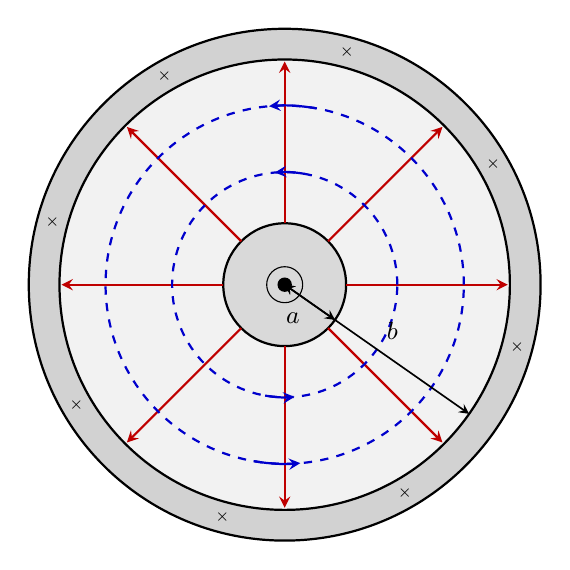
\begin{tikzpicture}[scale=1.3, >=latex]
		% --- СТИЛІ ЛІНІЙ ПОЛЯ ---
		\tikzset{
			Eline/.style={->, >=stealth, red!75!black, thick},
			Hline/.style={blue!80!black, thick, dashed},
			Harrow/.style={->, >=stealth, blue!80!black, solid, thick}
		}

		% --- ПРОВІДНИКИ ТА ДІЕЛЕКТРИК ---
		% Заповнення діелектрика між жилою та екраном
		\fill[gray!10] (0,0) circle (2.2);

		% Внутрішній провідник (жила)
		\fill[gray!30] (0,0) circle (0.6);
		\draw[thick] (0,0) circle (0.6);

		% Зовнішній провідник (екран)
		\fill[gray!35, even odd rule] (0,0) circle (2.5) (0,0) circle (2.2);
		\draw[thick] (0,0) circle (2.2);
		\draw[thick] (0,0) circle (2.5);

		% --- СТРУМИ В ПРОВІДНИКАХ ---
		% Струм "до спостерігача" у внутрішній жилі (\odot)
		\fill (0,0) circle (2pt);
		\draw (0,0) circle (5pt);

		% Струм "від спостерігача" у зовнішньому екрані (\otimes)
		\foreach \angle in {30, 75, 120, 165, 210, 255, 300, 345} {
			\node at (\angle:2.35) {\tiny $\times$};
		}

		% --- ЛІНІЇ ЕЛЕКТРИЧНОГО ПОЛЯ \Efield (РАДІАЛЬНІ) ---
		\foreach \angle in {0, 45, 90, 135, 180, 225, 270, 315} {
			\draw[Eline] (\angle:0.6) -- (\angle:2.18);
		}
		\node[red!75!black, above right] at (50:1.4) {$\Efield$};

		% --- ЛІНІЇ МАГНІТНОГО ПОЛЯ \Hfield (КОНЦЕНТРИЧНІ КОЛА) ---
		\foreach \r in {1.1, 1.75} {
			\draw[Hline] (0,0) circle (\r);
			% Стрілки напрямку магнітного поля (за правилом свердлика / правої руки)
			\draw[Harrow] (80:\r) arc (80:95:\r);
			\draw[Harrow] (260:\r) arc (260:275:\r);
		}
		\node[blue!80!black, above left] at (140:1.1) {$\Hfield$};

		% --- ПОЗНАЧЕННЯ РАДІУСІВ a та b ---
		\draw[<->, >=stealth, semithick] (0,0) -- (-35:0.6) node[midway, below left] {\small $a$};
		\draw[<->, >=stealth, semithick] (0,0) -- (-35:2.2) node[midway, above right] {\small $b$};

	\end{tikzpicture}
	\caption{Структура електромагнітного поля в поперечному перерізі довгої лінії (коаксіального кабелю): вектор $\Efield$ напрямлений від внутрішньої жили до зовнішнього екрана, а лінії вектора $\Hfield$ охоплюють провідник зі струмом.}
	\label{fig:line_cross_section}
\end{SCfigure}

Зауважимо важливу геометричну особливість поля в лінії:
\begin{itemize}
	\item Електричне поле $\Efield$ виникає через різницю потенціалів між провідниками, тому воно напрямлене \emphx{поперек} лінії (у площині $xy$).
	\item Магнітне поле $\Hfield$ створюється поздовжнім струмом $i(z,t)$ і закручене навколо провідників, тому воно також лежить \emphx{у поперечній площині} ($xy$).
\end{itemize}

Оскільки обидва вектори $\Efield$ та $\Hfield$ перпендикулярні до осі лінії $z$, таку хвилю називають \emphx{поперечною електромагнітною хвилею} (або ТЕМ-хвилею, керуючись теорією хвилеводів). Вектор Пойнтінга $\vect{S} = \frac{c}{4\pi} \left[ \Efield \times \Hfield \right]$, який описує густину потоку енергії, напрямлений точно вздовж осі $z$ --- від джерела до навантаження.

\begin{Attention}
	Провідники довгої лінії самі по собі не «проштовхують» енергію. Вони відіграють роль \emphx{напрямних елементів} (напрямної системи): задають граничні умови для електричного й магнітного полів, змушуючи електромагнітну хвилю поширюватися вздовж лінії. У цьому сенсі довга лінія є окремим випадком хвилеводу — а саме хвилеводу, який підтримує ТЕМ-хвилю. На відміну від порожнистих металевих хвилеводів, де ТЕМ-хвиля існувати не може, у довгій лінії наявність \emph{двох} провідників (або провідника й екрана) створює граничні умови, за яких існує поперечна електромагнітна хвиля з $\Efield \perp z$ та $\Hfield \perp z$.
\end{Attention}

\subsection{Фізичний зміст погонних параметрів $C_0$ та $L_0$}

Оскільки структура поля в кожному поперечному перерізі за формою збігається з відповідними задачами електростатики та магнітостатики, погонні параметри визначені суто геометрією провідників та властивостями діелектрика ($\varepsilon$, $\mu$).

З фундаментальних рівнянь Максвелла випливає універсальне співвідношення між погонною індуктивністю та ємністю для \emphx{довільної} лінії з двох провідників в однорідному середовищі:
\begin{equation}\label{eq:L0C0_universal}
	\tcbhighmath{
		L_0 C_0 = \varepsilon_0\epsilon \mu_0\mu.
	}
\end{equation}

Якщо підставити цей результат у формулу для фазової швидкості хвилі в лінії без втрат $v_{\text{ф}} = 1/\sqrt{L_0 C_0}$, ми отримаємо:
\begin{equation}\label{eq:phase_vel_maxwell}
	v_{\text{ф}} = \frac{1}{\sqrt{\epsilon_0 \mu_0\epsilon\mu}} = \frac{c}{\sqrt{\varepsilon \mu}},
\end{equation}
де $c = 1/\sqrt{\varepsilon_0 \mu_0}$ — швидкість світла у вакуумі.

Це фундаментальний результат: \emphx{сигнал у довгій лінії поширюється саме зі швидкістю світла у даному діелектрику}.

\subsection*{Приклад: Коаксіальний кабель}

Як приклад застосування польового підходу, розрахуємо параметри коаксіального кабелю з радіусом внутрішньої жили $a$, радіусом зовнішнього екрана $b$ та діелектриком ($\varepsilon$, $\mu$).

Застосовуючи теорему Гаусса та закон Ампера для перерізу кабелю:
\begin{equation}
	E(r) = \frac{q'}{2\pi\varepsilon r}, \qquad H(r) = \frac{i}{2\pi r},
\end{equation}
де $q'$ — погонний заряд. Знаходячи напругу $u = \int_a^b E(r)\,dr$ та магнітний потік $\Phi' = \int_a^b \mu H(r)\,dr$, отримуємо погонні параметри:
\begin{equation}
	C_0 = \frac{2\pi\varepsilon}{\ln(b/a)}, \qquad
	L_0 = \frac{\mu}{2\pi}\ln\left(\frac{b}{a}\right).
\end{equation}

Легко перевірити, що $L_0 C_0 = \varepsilon \mu$. Хвильовий опір такого кабелю $Z_{\text{хв}} = \sqrt{L_0/C_0}$ дорівнює:
\begin{equation}\label{eq:coax_impedance}
	Z_{\text{хв}} = \frac{1}{2\pi}\sqrt{\frac{\mu}{\varepsilon}} \ln\left(\frac{b}{a}\right) = \frac{\eta}{2\pi} \ln\left(\frac{b}{a}\right),
\end{equation}
де $\eta = \sqrt{\mu/\varepsilon}$ — хвильовий опір самого діелектрика (для вакууму $\eta_0 = \sqrt{\mu_0/\varepsilon_0} \approx 377~\text{Ом}$).